
\par Nuestra implementaci\'on de Task Batch consiste en crear un vector de bools de tama\~no $total\_cpu$ (el primer par\'ametro de la tarea), que se llena con $cant\_bloqueos$ valores en $true$ y el resto en $false$.
Luego, utilizamos el algoritmo de Fisher-Yates para hacer un shuffle del vector.
Finalmente, se lo recorre, y por cada posici\'on, si el valor es $true$ se hace una interrupci\'on de IO, y si es $false$ se hace uso de la CPU.
\par En la figura \ref{fig:figuraEj3} se puede ver un lote de tareas con 3 TaskBatch, con par\'ametros 5 y 2; 28 y 19; 14 y 13.
\begin{figure}[H]
\caption{Ejemplo de un lote de tareas con Task Batch}
\label{fig:figuraEj3}
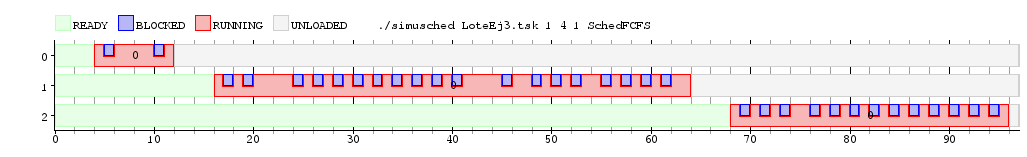
\includegraphics[width=1\textwidth]{imgs/imgEj3.png}
\end{figure}

